ブラウン運動とは、溶媒中の微粒子が溶媒分子の衝突によってランダムに運動する現象である。
ブラウン運動は次の
\begin{equation}\label{eq:brownian-motion}
	\odv{\bm{v}}{t} = \alpha \bm{v} + \bm{f}
\end{equation}
という運動方程式で表すことができる。
これを差分方程式化すると、
\begin{equation}
	\bm{v}_{t+1} = \left(1 - \dfrac{\alpha \Delta t}{m}\right) \bm{v}_t + \dfrac{\bm{f} \Delta t}{m}
\end{equation}
となり、漸化式を得る。
粒子は巨視的に見れば動かないことから平均速度が0と期待されること、
$f$が同一の分布に従うことなどから、
$\bm{v}$の分散は
\begin{equation}
	\ev{(v - \ev{v})^2} = \dfrac{\Delta t}{2 \alpha m} \ev{(f - \ev{f})^2}
\end{equation}
と書け、また気体分子運動論から$\ev{v^2} = \dfrac{kT}{m}$であることを考慮すると、
\begin{equation}
	\ev{(f - \ev{f})^2} = \dfrac{2 \alpha k T}{\Delta t}
\end{equation}
となる。
よって、平均0、分散が$\dfrac{2 \alpha k T}{\Delta t}$の正規分布に従う乱数を用いることで、\footnote{
	結局、$v$を正規分布に従う乱数で更新してもよく、
	\begin{equation}
		x_{t+1} = x_t + \mathcal{N}
	\end{equation}
	としてもよい。
	この場合は、オーダーに注意である。
}
$v$を計算し、
\begin{equation}
	\bm{r}_{t+1} = \bm{r}_t + \bm{v} \Delta t
\end{equation}
で位置を更新すれば、ブラウン運動をシミュレーションすることができる。\footnote{
	詳しくは\cite{brownian-motion-report}課題8を参照
}

実際に、この方法でブラウン運動をシミュレーションし、その結果を図\ref{fig:brownian-2d-sim}に示す。
\begin{figure}
	\centering
	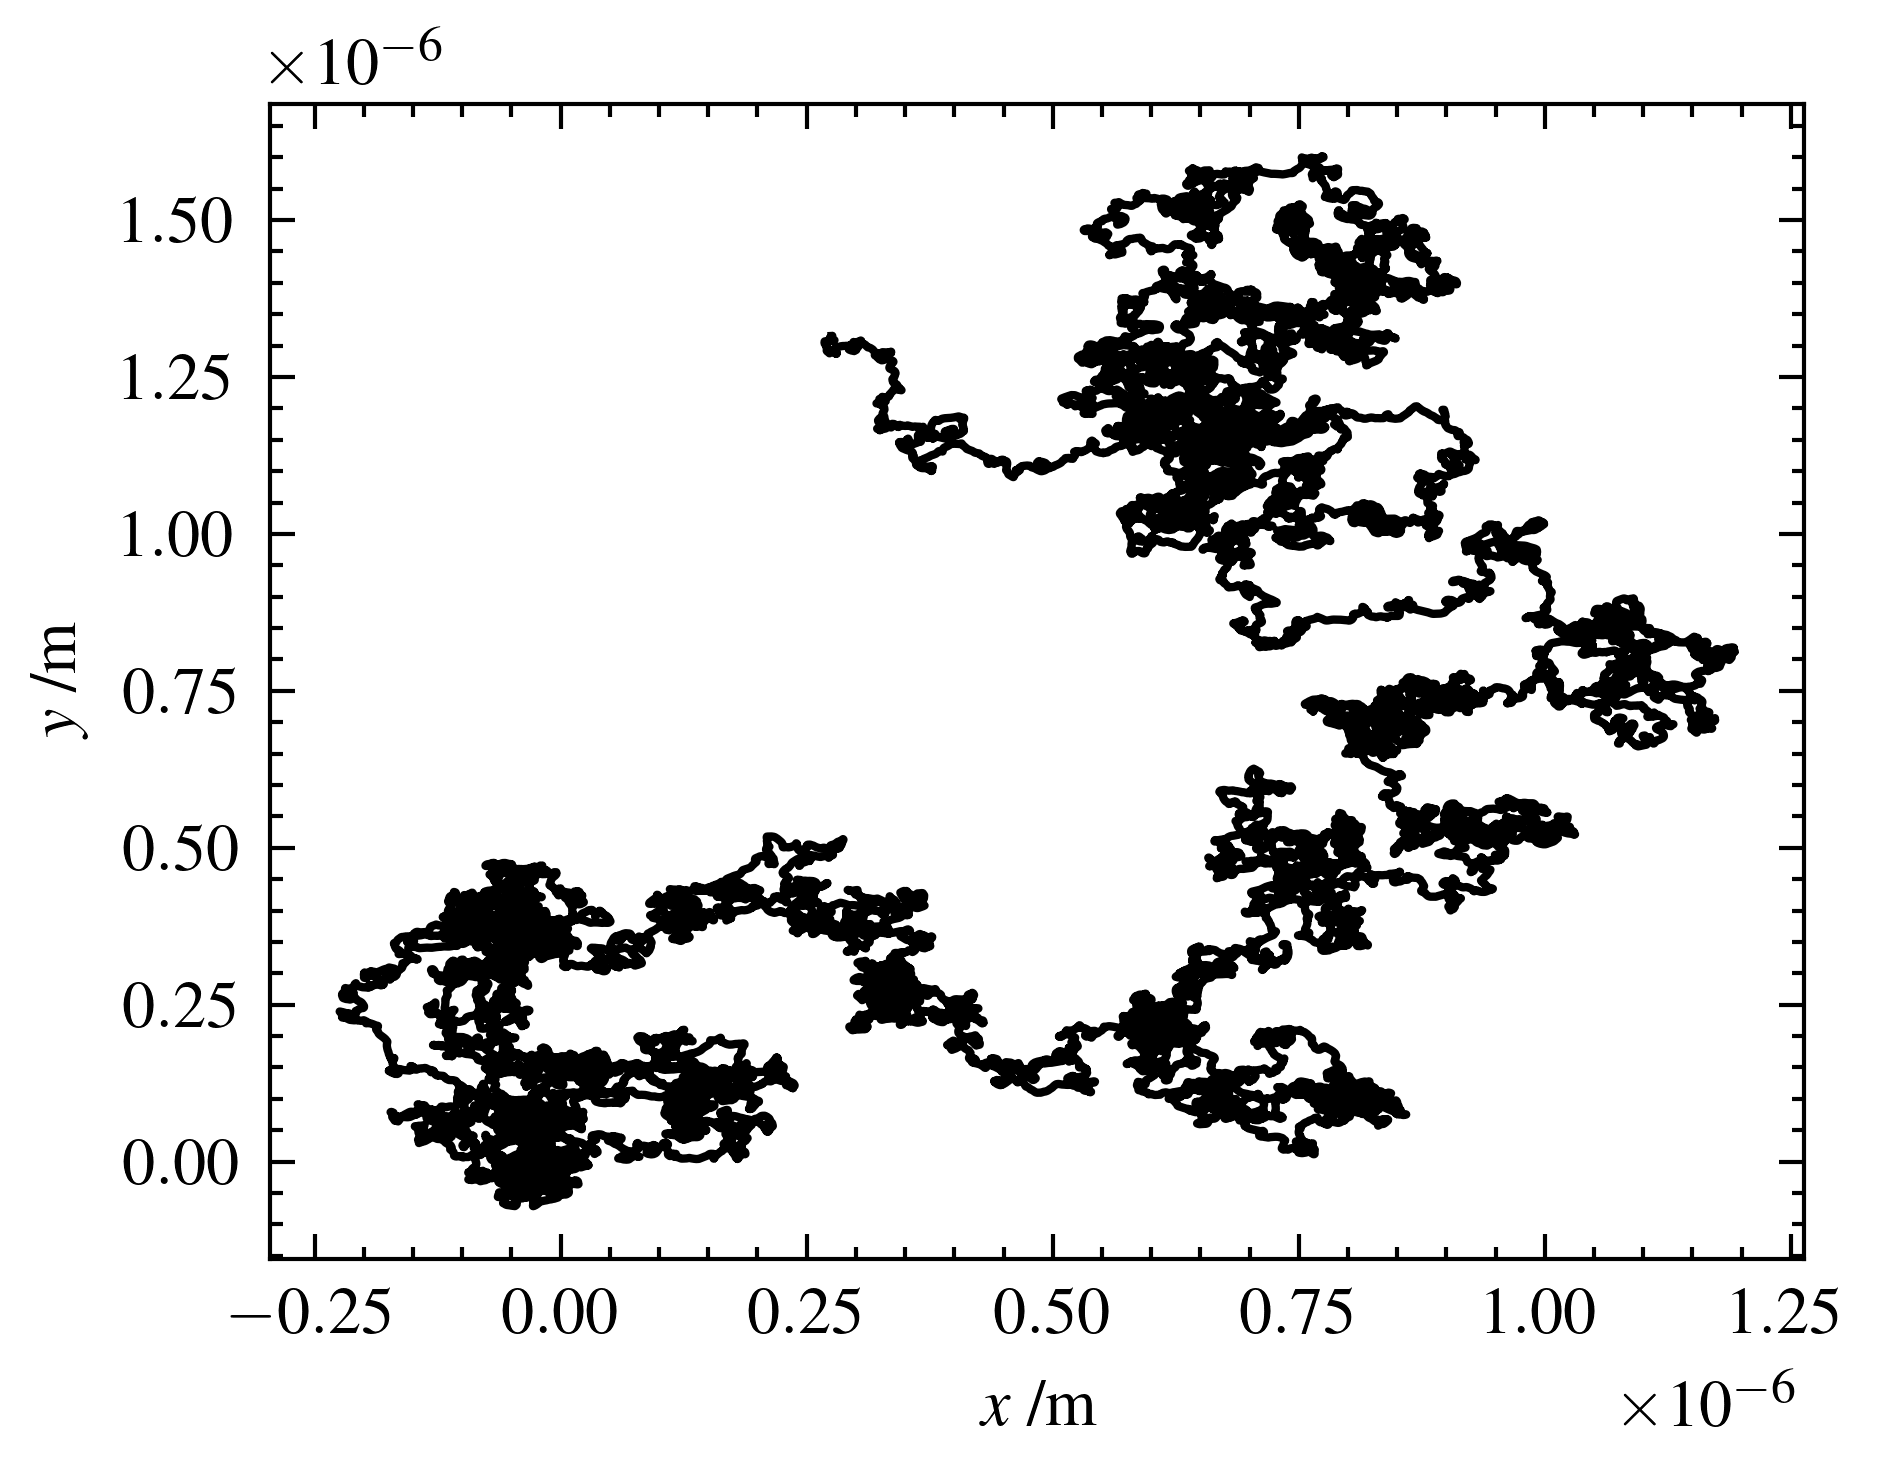
\includegraphics[width=0.8\linewidth]{./src/figures/brownian-2d-sim/brownian-2d-sim.png}
	\caption{2次元ブラウン運動のシミュレーション}\label{fig:brownian-2d-sim}
\end{figure}

